%% (Master) Thesis template
% Template version used: v1.4
%
% Largely adapted from Adrian Nievergelt's template for the ADPS
% (lecture notes) project.


%% We use the memoir class because it offers a many easy to use features.
\documentclass[11pt,a4paper]{memoir}

%% Packages
%% ========

%% LaTeX Font encoding -- DO NOT CHANGE
\usepackage[OT1]{fontenc}

%% Babel provides support for languages.  'english' uses British
%% English hyphenation and text snippets like "Figure" and
%% "Theorem". Use the option 'ngerman' if your document is in German.
%% Use 'american' for American English.  Note that if you change this,
%% the next LaTeX run may show spurious errors.  Simply run it again.
%% If they persist, remove the .aux file and try again.
\usepackage[english]{babel}

%% Input encoding 'utf8'. In some cases you might need 'utf8x' for
%% extra symbols. Not all editors, especially on Windows, are UTF-8
%% capable, so you may want to use 'latin1' instead.
\usepackage[utf8]{inputenc}

%% This changes default fonts for both text and math mode to use Herman Zapfs
%% excellent Palatino font.  Do not change this.
\usepackage[sc]{mathpazo}

%% The AMS-LaTeX extensions for mathematical typesetting.  Do not
%% remove.
\usepackage{amsmath,amssymb,amsfonts,mathrsfs}

%% NTheorem is a reimplementation of the AMS Theorem package. This
%% will allow us to typeset theorems like examples, proofs and
%% similar.  Do not remove.
%% NOTE: Must be loaded AFTER amsmath, or the \qed placement will
%% break
\usepackage[amsmath,thmmarks]{ntheorem}

%% LaTeX' own graphics handling
\usepackage{graphicx}

%% We unfortunately need this for the Rules chapter.  Remove it
%% afterwards; or at least NEVER use its underlining features.
\usepackage{soul}

%% This allows you to add .pdf files. It is used to add the
%% declaration of originality.
\usepackage{pdfpages}

%% Some more packages that you may want to use.  Have a look at the
%% file, and consult the package docs for each.
%% See the TeXed file for more explanations

%% [OPT] Multi-rowed cells in tabulars
%\usepackage{multirow}

%% [REC] Intelligent cross reference package. This allows for nice
%% combined references that include the reference and a hint to where
%% to look for it.
\usepackage{varioref}

%% [OPT] Easily changeable quotes with \enquote{Text}
%\usepackage[german=swiss]{csquotes}

%% [REC] Format dates and time depending on locale
\usepackage{datetime}

%% [OPT] Provides a \cancel{} command to stroke through mathematics.
%\usepackage{cancel}

%% [NEED] This allows for additional typesetting tools in mathmode.
%% See its excellent documentation.
\usepackage{mathtools}

%% [ADV] Conditional commands
%\usepackage{ifthen}

%% [OPT] Manual large braces or other delimiters.
%\usepackage{bigdelim, bigstrut}

%% [REC] Alternate vector arrows. Use the command \vv{} to get scaled
%% vector arrows.
\usepackage[h]{esvect}

%% [NEED] Some extensions to tabulars and array environments.
\usepackage{array}

%% [OPT] Postscript support via pstricks graphics package. Very
%% diverse applications.
%\usepackage{pstricks,pst-all}

%% [?] This seems to allow us to define some additional counters.
%\usepackage{etex}

%% [ADV] XY-Pic to typeset some matrix-style graphics
%\usepackage[all]{xy}

%% [OPT] This is needed to generate an index at the end of the
%% document.
%\usepackage{makeidx}

%% [OPT] Fancy package for source code listings.  The template text
%% needs it for some LaTeX snippets; remove/adapt the \lstset when you
%% remove the template content.
\usepackage{listings}
\lstset{language=TeX,basicstyle={\normalfont\ttfamily}}

%% [REC] Fancy character protrusion.  Must be loaded after all fonts.
\usepackage{microtype}

%% [REC] Nicer tables.  Read the excellent documentation.
\usepackage{booktabs}


%% Our layout configuration.  DO NOT CHANGE.
%% Memoir layout setup

%% NOTE: You are strongly advised not to change any of them unless you
%% know what you are doing.  These settings strongly interact in the
%% final look of the document.

% Dependencies
\usepackage{ETHlogo}

% Turn extra space before chapter headings off.
\setlength{\beforechapskip}{0pt}

\nonzeroparskip
\parindent=0pt
\defaultlists

% Chapter style redefinition
\makeatletter

\if@twoside
  \pagestyle{Ruled}
  \copypagestyle{chapter}{Ruled}
\else
  \pagestyle{ruled}
  \copypagestyle{chapter}{ruled}
\fi
\makeoddhead{chapter}{}{}{}
\makeevenhead{chapter}{}{}{}
\makeheadrule{chapter}{\textwidth}{0pt}
\copypagestyle{abstract}{empty}

\makechapterstyle{bianchimod}{%
  \chapterstyle{default}
  \renewcommand*{\chapnamefont}{\normalfont\Large\sffamily}
  \renewcommand*{\chapnumfont}{\normalfont\Large\sffamily}
  \renewcommand*{\printchaptername}{%
    \chapnamefont\centering\@chapapp}
  \renewcommand*{\printchapternum}{\chapnumfont {\thechapter}}
  \renewcommand*{\chaptitlefont}{\normalfont\huge\sffamily}
  \renewcommand*{\printchaptertitle}[1]{%
    \hrule\vskip\onelineskip \centering \chaptitlefont\textbf{\vphantom{gyM}##1}\par}
  \renewcommand*{\afterchaptertitle}{\vskip\onelineskip \hrule\vskip
    \afterchapskip}
  \renewcommand*{\printchapternonum}{%
    \vphantom{\chapnumfont {9}}\afterchapternum}}

% Use the newly defined style
\chapterstyle{bianchimod}

\setsecheadstyle{\Large\bfseries\sffamily}
\setsubsecheadstyle{\large\bfseries\sffamily}
\setsubsubsecheadstyle{\bfseries\sffamily}
\setparaheadstyle{\normalsize\bfseries\sffamily}
\setsubparaheadstyle{\normalsize\itshape\sffamily}
\setsubparaindent{0pt}

% Set captions to a more separated style for clearness
\captionnamefont{\sffamily\bfseries\footnotesize}
\captiontitlefont{\sffamily\footnotesize}
\setlength{\intextsep}{16pt}
\setlength{\belowcaptionskip}{1pt}

% Set section and TOC numbering depth to subsection
\setsecnumdepth{subsection}
\settocdepth{subsection}

%% Titlepage adjustments
\pretitle{\vspace{0pt plus 0.7fill}\begin{center}\HUGE\sffamily\bfseries}
\posttitle{\end{center}\par}
\preauthor{\par\begin{center}\let\and\\\Large\sffamily}
\postauthor{\end{center}}
\predate{\par\begin{center}\Large\sffamily}
\postdate{\end{center}}

\def\@advisors{}
\newcommand{\advisors}[1]{\def\@advisors{#1}}
\def\@department{}
\newcommand{\department}[1]{\def\@department{#1}}
\def\@thesistype{}
\newcommand{\thesistype}[1]{\def\@thesistype{#1}}

\renewcommand{\maketitlehooka}{\noindent\ETHlogo[2in]}

\renewcommand{\maketitlehookb}{\vspace{1in}%
  \par\begin{center}\Large\sffamily\@thesistype\end{center}}

\renewcommand{\maketitlehookd}{%
  \vfill\par
  \begin{flushright}
    \sffamily
    \@advisors\par
    \@department, ETH Z\"urich
  \end{flushright}
}

\checkandfixthelayout

\setlength{\droptitle}{-48pt}

\makeatother

% This defines how theorems should look. Best leave as is.
\theoremstyle{plain}
\setlength\theorempostskipamount{0pt}

%%% Local Variables:
%%% mode: latex
%%% TeX-master: "thesis"
%%% End:


%% Theorem environments.  You will have to adapt this for a German
%% thesis.
%% Theorem-like environments

%% This can be changed according to language. You can comment out the ones you
%% don't need.

\numberwithin{equation}{chapter}

%% German theorems
%\newtheorem{satz}{Satz}[chapter]
%\newtheorem{beispiel}[satz]{Beispiel}
%\newtheorem{bemerkung}[satz]{Bemerkung}
%\newtheorem{korrolar}[satz]{Korrolar}
%\newtheorem{definition}[satz]{Definition}
%\newtheorem{lemma}[satz]{Lemma}
%\newtheorem{proposition}[satz]{Proposition}

%% English variants
\newtheorem{theorem}{Theorem}[chapter]
\newtheorem{example}[theorem]{Example}
\newtheorem{remark}[theorem]{Remark}
\newtheorem{corollary}[theorem]{Corollary}
\newtheorem{definition}[theorem]{Definition}
\newtheorem{lemma}[theorem]{Lemma}
\newtheorem{proposition}[theorem]{Proposition}

%% Proof environment with a small square as a "qed" symbol
\theoremstyle{nonumberplain}
\theorembodyfont{\normalfont}
\theoremsymbol{\ensuremath{\square}}
\newtheorem{proof}{Proof}
%\newtheorem{beweis}{Beweis}


%% Helpful macros.
%% Custom commands
%% ===============

%% Special characters for number sets, e.g. real or complex numbers.
\newcommand{\C}{\mathbb{C}}
\newcommand{\K}{\mathbb{K}}
\newcommand{\N}{\mathbb{N}}
\newcommand{\Q}{\mathbb{Q}}
\newcommand{\R}{\mathbb{R}}
\newcommand{\Z}{\mathbb{Z}}
\newcommand{\X}{\mathbb{X}}

%% Fixed/scaling delimiter examples (see mathtools documentation)
\DeclarePairedDelimiter\abs{\lvert}{\rvert}
\DeclarePairedDelimiter\norm{\lVert}{\rVert}

%% Use the alternative epsilon per default and define the old one as \oldepsilon
\let\oldepsilon\epsilon
\renewcommand{\epsilon}{\ensuremath\varepsilon}

%% Also set the alternate phi as default.
\let\oldphi\phi
\renewcommand{\phi}{\ensuremath{\varphi}}


%% Make document internal hyperlinks wherever possible. (TOC, references)
%% This MUST be loaded after varioref, which is loaded in 'extrapackages'
%% above.  We just load it last to be safe.
\usepackage[linkcolor=black,colorlinks=true,citecolor=black,filecolor=black]{hyperref}

%\let\endtitlepage\relax % no empty page after title, TODO remove

% \renewcommand\textbullet{\ensuremath{\bullet}}
\usepackage{newtxtext,newtxmath}

%% Document information
%% ====================

\title{Enclave Hardening for Privacy Preserving Machine Learning}
\author{Rudolf Loretan}
\thesistype{Master Thesis}
\advisors{Advisors: Dr.\ K. Kostiainen, Prof.\ Dr.\ E. Mohammadi}
\department{Department of Computer Science}
\date{November 17, 2021}

\begin{document}

\frontmatter

%% Title page is autogenerated from document information above.  DO
%% NOT CHANGE.

\AtBeginShipoutNext{\AtBeginShipoutNext{\AtBeginShipoutDiscard}} % TODO, this temporarily removes blank page after title
\begin{titlingpage}
  \calccentering{\unitlength}
  \begin{adjustwidth*}{\unitlength-24pt}{-\unitlength-24pt}
    \maketitle
  \end{adjustwidth*}
\end{titlingpage}

%% high level overview
% \begin{itemize}
  \item This example thesis briefly shows the main features of our thesis
  style, and how to use it for your purposes.
  \item This example thesis briefly shows the main features of our thesis
  style, and how to use it for your purposes.
  \item This example thesis briefly shows the main features of our thesis
  style, and how to use it for your purposes.
\end{itemize}




%% The abstract of your thesis.  Edit the file as needed.
\clearpage
\begin{abstract}
  Cyber risk assessment is an emerging field, in particular for insurance companies, that offer cyber insurance packages to their clients. However, understanding cyber risk is not easy, especially due to the lack of historical data. While machine learning can help, reconciling accuracy, explainability and privacy when data is lacking is challenging. Some machine learning techniques are better than others at addressing these challenges. For instance, ensemble methods such as gradient boosted decision trees (GBDT) are easily explainable, due to their tree structure. This is not the case of other methods such as deep neural networks, which are much more complex to interpret. GBDT models can also provide privacy through differential privacy. However, current state of the arts on differentially private GBDT models suffers from low accuracy when there are limited training data. In this thesis, we propose a new decision tree induction algorithm, \textit{2-nodes}, that enhances accuracy over small datasets while satisfying $\epsilon$-differential privacy. Further, we propose an algorithm based on Bayesian networks to generate synthetic data for cyber risk assessment. Finally, we evaluate our model on various real and synthetic datasets and show that our new induction method is able to improve accuracy on small datasets.
  \end{abstract}

\clearpage

%% TOC with the proper setup, do not change.
%\cleartorecto
\tableofcontents
\mainmatter

%% Your real content!
\chapter{Introduction}

\section{Motivation}

In many scenarios where machine learning (ML) is involved, the responsible developing team strives to have an accurate, explainable model. Accurate, because the end goal of an ML model is to help the team in understanding a problem better. Inaccurate outputs would not be helpful. Explainable, because if the team cannot understand the decisions made by the model, in particular the steps involved in these decisions, the problem would remain as complex as it was. Any machine learning model needs a starting point. This starting point usually takes the form of a \textit{training set}. 

The training set contains data about the problem to be learned about, and sometimes data about the solution to be found (\textit{unsupervised} vs. \textit{supervised} learning). In some cases, leakage of the training data creates serious privacy issues, which for some applications is unacceptable. This leads the model to not only require being accurate and explainable, but also to prevent such privacy leaks. One way to prevent these leaks is to train the model in a privacy preserving fashion. Privacy preserving machine learning models can offer guarantees that prevent information about the training data to be extracted. An example application where privacy of the training data is important can be found in assessing \textit{cyber risk}, which we focus on in this thesis.

In recent years, cyber attacks and data breaches have surged, as outlined by recent reports (\cite{verizon_report}, \cite{ibm_report}, \cite{cisco_report}). Companies, large and small, have an increasing need for protection. Such protection not only extends to their technical infrastructure and ability to respond to incidents, but also to potential financial losses that they may face. To cover the latter, insurance companies have come up with cyber insurance products. From the insurer perspective's however, assessing the cyber risk that a particular customer is exposed to is highly challenging. The understanding of cyber risk, i.e. how to describe or model the risk, is not yet as understood as other risks, such as the ones covered by car insurance products.

One major issue that insurers face is trustworthiness when it comes to data provided by their customers. Indeed, customers are often unwilling to disclose their true security practices, fearing that such information could be used to discriminate against them, should they not be complying with or implementing these practices according to the latest industry standards. Currently, these information are collected by insurers through questionnaires that the customers need to fill in. These questionnaires will typically include questions about their security management practices, e.g. details about their software patching process or remote access policy.

\section{Example setting}

One way to address above problems is for insurers to give customers access to an interface allowing them to answer their questionnaires, within a protected space (such as an Intel SGX enclave). This protected space:

\begin{itemize}
	\item can be used to collect sensitive data, while reassuring both the insurers and the customers that no party has direct access to the data.
	\item can be leveraged by customers through remote attestation to verify the correctness of the protected space (i.e. the integrity of any code running within the enclave).
	\item can give customers privacy guarantees with respect to the data they provide.
\end{itemize}

This is represented on the left hand side of Figure ~\ref{fig:big_picture}. In this thesis, we focus on enabling a trustworthy evaluation of the data collected within the protected space. The goal of this evaluation is to train a machine learning model that can be used by insurers to help them evaluate the risk and potential losses associated to the onboarding of a new customer, while providing customers peace of mind about their data. This is represented on the right hand side of Figure ~\ref{fig:big_picture}.

\begin{figure}[h!]
	\center
	\includegraphics[scale=0.75]{images/introduction/big_picture}
	\caption{\label{fig:big_picture} The SGX application on the left hand side, and the privacy preserving machine learning operating within the SGX enclave, zoomed in on the right hand side. SGX application schematic adapted from \cite{sgx_fig}.}
\end{figure}

The insurance company hosts the enclave. The data that the customers send are sent encrypted to the enclave, and never leave it. The data cannot be queried directly, be it by the customers or the insurance company. The SGX enclave can then release the trained model to the insurance company, which can leverage it to learn various kinds of information about the customers. However, due to the privacy preserving properties of the model, the insurance company cannot retrieve information about any single customer.



\section{Chosen approach}

Gradient Boosted Decision Tree (GBDT) models have attracted a lot of attention in recent years and have successfully been used as a winning model in various machine learning competitions\footnote{\href{https://github.com/dmlc/xgboost/tree/master/demo\#machine-learning-challenge-winning-solutions}{https://github.com/dmlc/xgboost/tree/master/demo\#machine-learning-challenge-winning-solutions}}. GBDT models have been shown to be performant, and easily explainable due to their tree structure. In addition, research work (e.g. of Qinbin et al. (2020) \cite{dpgbdt} or Liu et al. (2018) \cite{liu}) has pushed GBDT models towards becoming privacy preserving by leveraging differential privacy. While differential privacy is not the only way to provide privacy (see Chapter ~\ref{chap:related_work}), its strong mathematical foundations and provable properties have made it a de-facto choice in many research work. Although our example setting justifies the attack model that we consider in Chapter ~\ref{chap:security_analysis}, this thesis focuses on the improvement and evaluation of the algorithmic parts: differential privacy applied to gradient boosted decision trees.

\section{Contributions}

While recent work shows encouraging results, developing gradient boosted decision tree models that satisfy $\epsilon$-differential privacy while remaining as accurate as non-private models is still an open challenge, especially when the training data is small, such as in the case of cyber risk evaluation. This thesis aims at addressing the current shortcomings of previous approachs, with the following contributions:

\begin{enumerate} 
	\item We propose a new decision tree induction method, called \textit{2-nodes}, that enhances accuracy over low-populated datasets, while satisfying $\epsilon$-differential privacy. In particular, we propose to make use of extra data in the tree induction process, by finding the optimal splitting point over a node and its sibling's data rather than just the node itself. We use this induction method in an implementation of DP-GBDT that we implement from the literature. This is covered in Chapter ~\ref{chap:2-nodes}.

	\item In Chapter ~\ref{chap:synthetic_data}, and since real data is lacking, we propose a way to generate synthetic datasets that mimic cyber insurance questionnaire answers. To achieve this, we collect figures from cyber security reports written by different vendors in the security and insurance sector, and derive a Bayesian network that we use to compute the dataset's features and targets.

	\item We show in Chapter ~\ref{sec:evaluation} that our model can successfully be used to accurately evaluate cyber risk on 4 different synthetic datasets, as well as improve predictions over low-populated datasets. 
	
	\item We explore privacy attacks on machine learning models in Chapter ~\ref{chap:security_analysis} and apply them to our DP-GBDT model, and show that in some cases it can reduce attack accuracy under strong privacy constraints.
\end{enumerate}


\chapter{Background}

\section{Gradient boosted decision trees (GBDT)}

Dummy text.

\section{Differential privacy}

Dummy text.

\section{Differentially private gradient boosted decision trees (DP-GBDT)}

Dummy text.

\section{Intel SGX}

Dummy text.

\section{Side channels}

Dummy text.
\chapter{Security Analysis}\label{chap:security_analysis}

\section{Attack landscape}

In this section, we give an overview of the various attacks that we consider for our model.

\subsection{Enclave attacks}

Most SGX attacks are side-channel \cite{sgx_survey} attacks, i.e. attacks that are based on information gained from the implementation of the system under attack, rather than weaknesses in the implementation itself. Popular side-channel attacks against SGX are cache-based timing attacks, such as \textit{Flush+Reload} \cite{flush_reload} or \textit{Prime+Probe} \cite{prime_probe}. Both attacks exploit cache behaviour to leak information on victim access to shared memory. In \textit{Flush+Reload}, the attacker flushes a memory line and then measures the time that it takes for the line to be reloaded. If the line was reloaded fast, then the attacker infers that the victim accessed the data located at that line. In \textit{Prime+Probe}, the attacker first primes the cache (i.e. loads it with dummy data) and waits for the victim to access one of the cache lines. Afterwards, the attacker probes the cache and measures its response time. If the access is fast, then the victim did not access this cache line. If it is slow, it did access it. Figure ~\ref{fig:cache} shows how processors fetch data from the cache / memory, and how it relates to access time.

To defend against such attacks, the enclave's authors must make sure that their design is side-channel resilient. This can be achieved by making sure that the code is designed in a cache leakage-free manner, making the execution flow and memory access patterns independent of the data accessed. For other kinds of attacks, \cite{sgx_survey} suggests that authors can act on multiple fronts: microcode patches, system/application design and compiler/SDK. While this is an active and interesting research area, it is mostly independent of the focus of this thesis, and thus we will not explore these attacks further.

\begin{figure}[h!]
	\center
	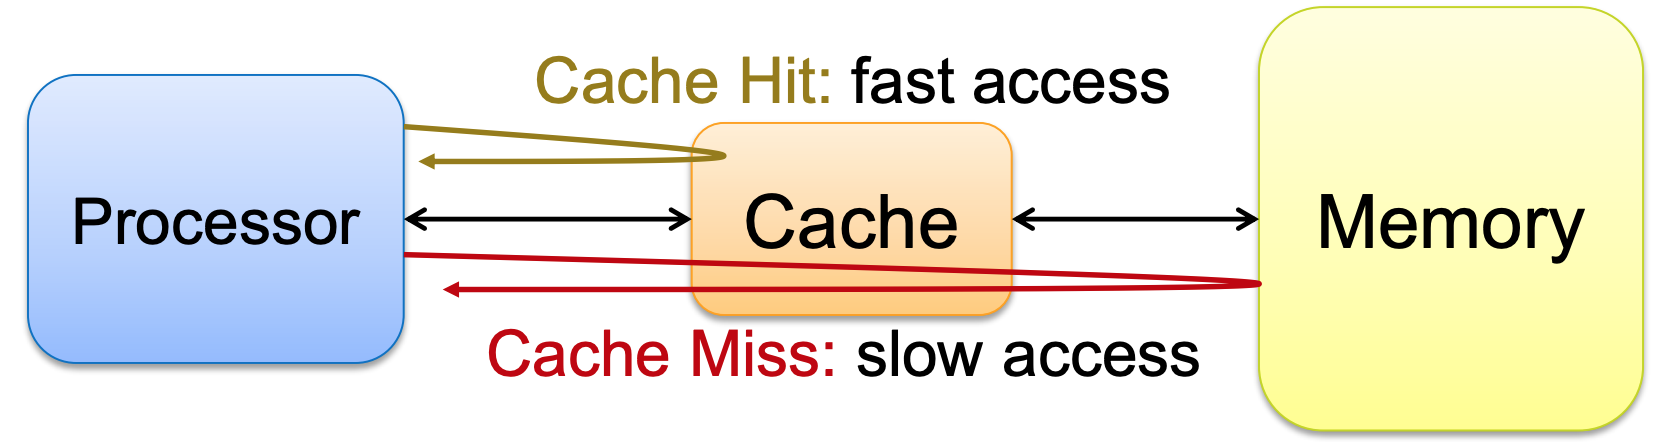
\includegraphics[scale=0.35]{images/introduction/cache}
	\caption{\label{fig:cache} Illustration of a processor fetching data from cache or memory \cite{intel_slides}.}
\end{figure}

\subsection{Security \& privacy attacks}

Since the questionnaires are served to the customers through e.g. a web application, we must consider security attacks targeted at such applications. A malicious customer could try to influence the model accuracy by tempering with the learning set. This could be done by e.g. flooding the web application with bogus questionnaire's answers. In this thesis we will assume that customers are trustworthy, and we will instead focus on privacy attacks, in particular those that target machine learning models.

If a machine learning model was trained using personal data, such as people's health records or identity information, then a privacy attack would aim at extracting these information to benefit the attacking party. For the scope of this thesis, we consider the insurance company to be the adversary, since they own the machine learning model. While they cannot access its content (as it is enclave-protected), it can design privacy attacks in order to gain information about the training set used by the model (i.e. the questionnaires submitted by the customers). Since it is assumed that the model is trained and run within a trusted environment, we will focus our threat model on black-box attacks (i.e. the attacker only has access to the model's API, can submit input vectors and retrieve their corresponding predictions), as shown in Figure ~\ref{fig:threat_model} (adapted from \cite{ml_survey}).

\begin{figure}[h!]
	\center
	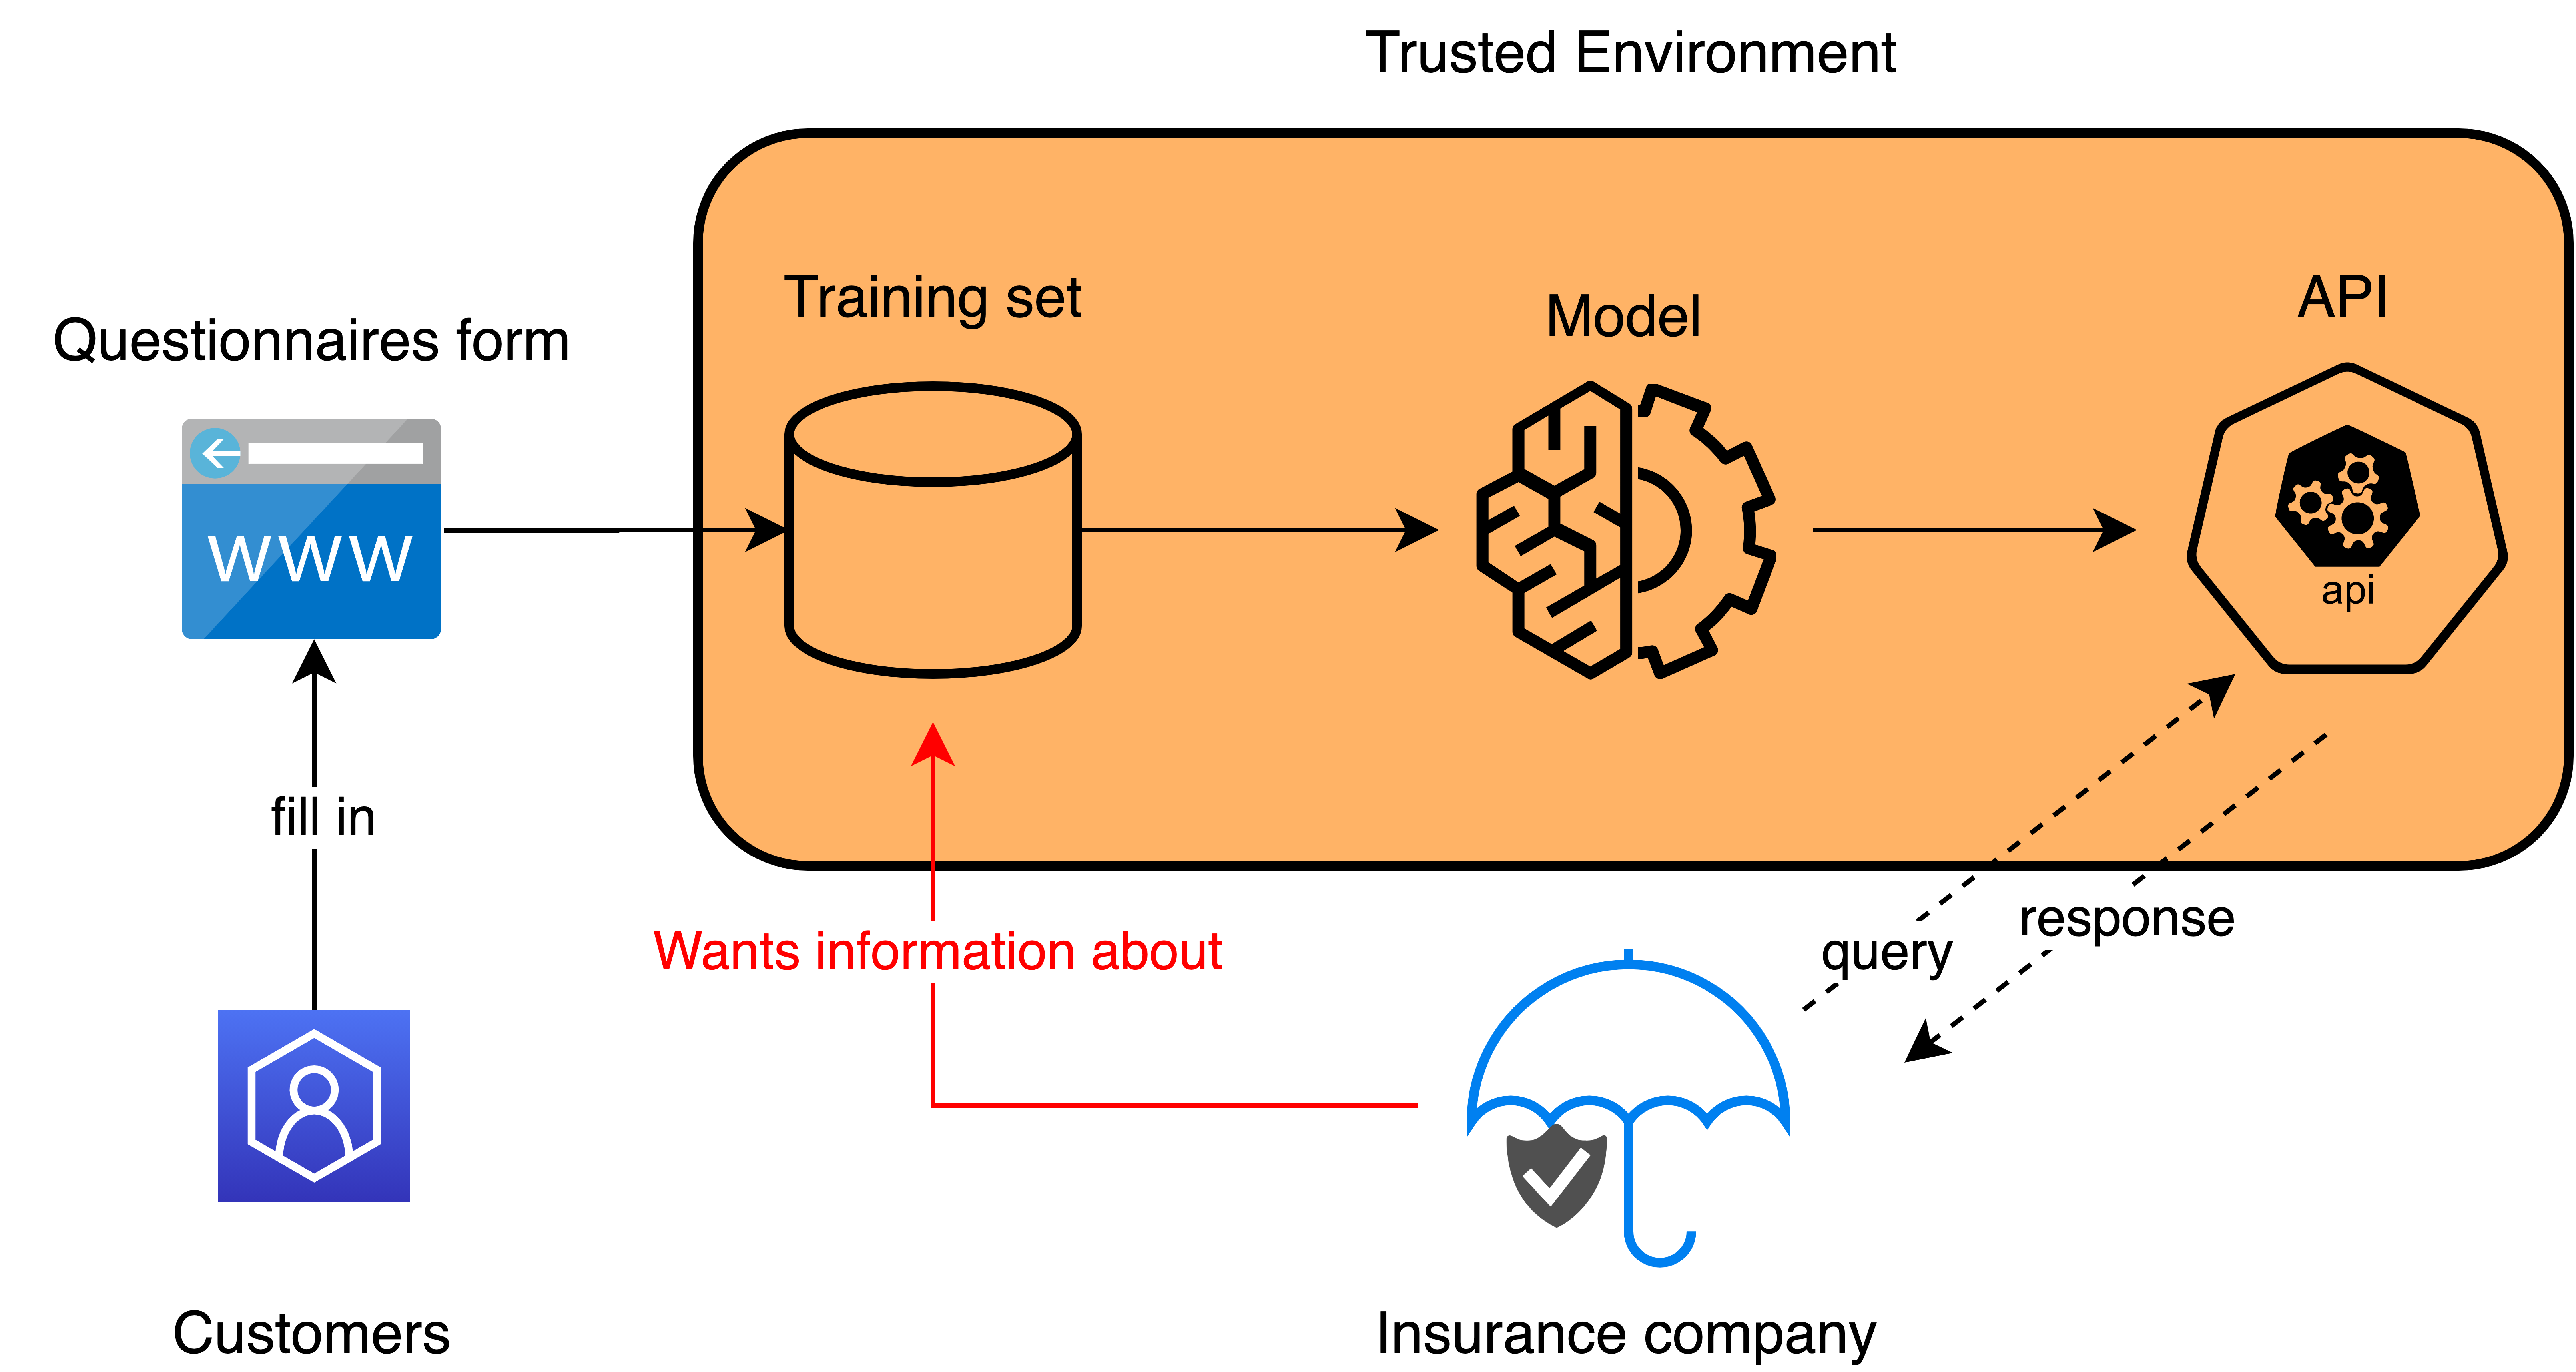
\includegraphics[scale=0.76]{images/introduction/threat_model}
	\caption{\label{fig:threat_model} Threat model}
\end{figure}

In such a model, the insurance company is interested in gaining meaningful information about the training instances that were used by the model. Several attacks can be constructed \cite{ml_survey}:

\begin{itemize}
	\item \textbf{Membership inference attack}: these attacks aim at determining whether or not an input vector $\mathbf{x}$ was used as part of the training set. First introduced by Shokri et al. (2017) \cite{shokri}, it is one of the most popular attacks. This attack assumes a black-box scenario where the attacker only has access to the prediction vectors.
	\item \textbf{Model inversion attack}: given a prediction vector $\mathbf{\hat{y}}$ and partial knowledge of some features of the initial sample $\mathbf{x}$, this attack aims at recovering information about one or all missing features. This is not to be confused with \textit{attribute inference attacks}, which try to infer sensitive feature's values of a targeted instance by leveraging publicly available data.
	\item \textbf{Property inference attack}: these attacks aim at extracting properties over the training set that were not explicitly encoded as features during the learning task. For instance, our synthetic data generation process (described in details in Chapter ~\ref{chap:synthetic_data}) does not encode the number of employees of a company in the dataset. Trying to determine such property from the model would fall under this category of attacks.
	\item \textbf{Model extraction attack}: these attacks do not aim at recovering information about the training dataset, but information about the inner working of the learning model, in order to reconstruct a substitute model that behaves similarly.
\end{itemize}

Many of the above attacks are conducted through \textit{shadow models training}, which is illustrated in Figure ~\ref{fig:shadow}. In shadow training, the attacker trains various models (the so-called shadow models) on shadow datasets, i.e. datasets that follow a similar distribution as the target dataset. Once the shadow models are trained, the attacker constructs an attack dataset, where each instance typically represents the probability vector outputted by the shadow models. The attacker can then train an attack model, which takes as input a prediction vector and outputs membership / property information.

\begin{figure}[h!]
	\center
	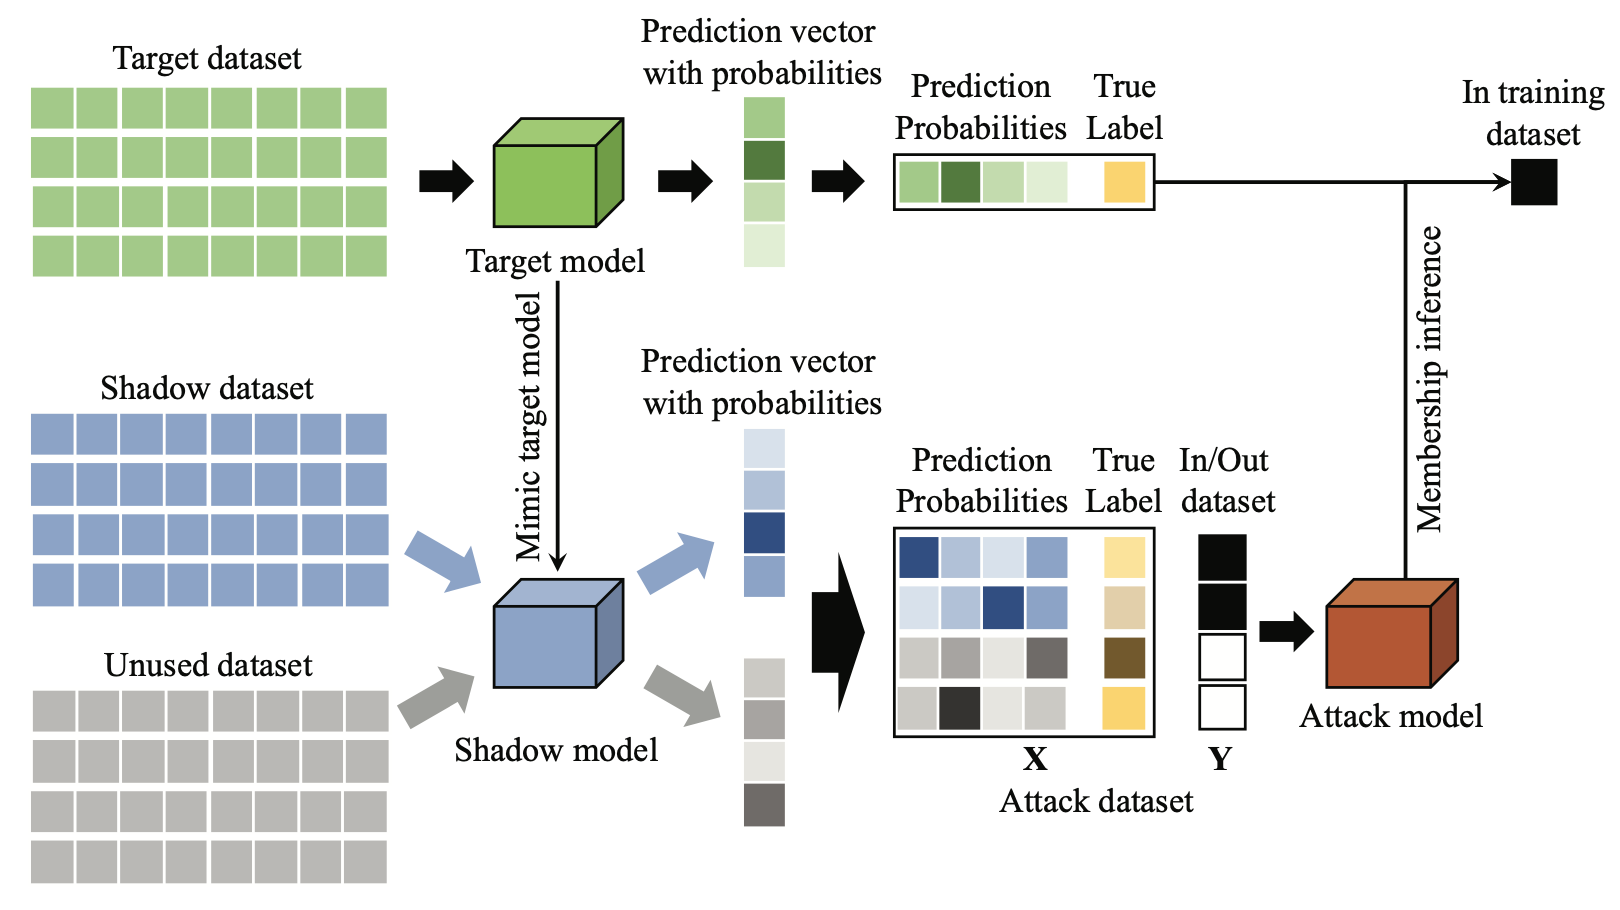
\includegraphics[scale=0.52]{images/introduction/mia}
	\caption{\label{fig:shadow} Shadow training architecture for a membership inference attack. \cite{chen}}
\end{figure}

\section{Attacks on DP-GBDT}

While there are many Python libraries readily available to conduct privacy attacks on machine learning models, such as the \textit{adversarial-robustness-toolbox} Python library\footnote{\href{https://github.com/Trusted-AI/adversarial-robustness-toolbox}{https://github.com/Trusted-AI/adversarial-robustness-toolbox}}, to the best of our knowledge there is no work in the literature that considers privacy attacks on regression models such as our ensemble of gradient boosted decision trees. We therefore tried to convert our synthetic datasets to a classification task, and to tweak our model to support multi-class classification. We evaluate several classical attacks, in particular the gap attack, introduced by Shokri et al. (2017) \cite{shokri}, for different train-test split ratios. Unfortunately, our tests indicate that the current attacks do not adapt well to regression models. In particular, we were unable to detect an explainable correlation between the privacy budget and the accuracy of the membership inference attack. For reference, our results are shown in Figure ~\ref{fig:attack_cost} and summarised in Table ~\ref{table:attack_cost} (for a fixed $\epsilon=0.1$). 

While for low $\epsilon$ values, our model is effectively reducing the success rate of membership inference attacks to $60\%$ or below, the literature (\cite{chen}, \cite{label_only}) shows that we should see such values starting from a higher $\epsilon$ value. Figure ~\ref{fig:attack_cost_50} shows the same attack on a 50-50\% train-test split. From the Figure, what happens is unclear: the model seems not to be leaking any data. However this should be interpreted with a grain of salt, as this could be the result of a lack of better attacks for GBDT models. Indeed, most of current work that evaluates the impact of differential privacy on membership inference attacks targets neural networks and deep learning models only (such as the work in \cite{chen} and \cite{dp_mia}). The reader can refer to Figure 4 in \cite{ref_attack} to get an idea of the influence of differential privacy against membership inference attacks for neural networks.

During this thesis, we have also tried to evaluate the model against other inference attacks, such as attribute inference attacks. Different settings were tested, such as growing very deep decision trees to overfit on the training data. This was done using both the \textit{adversarial-robustness-toolbox} as well as other work found on popular open-source website GitHub. Results were hovering in the 50\% attack accuracy zone, consistently across the different tools, confirming that our model could not be evaluated as-is. This shows that developing privacy attacks on regression ensemble models will be an important step in evaluating them, and we encourage future work in that direction.
\chapter{Methods and Implementation}

\section{Assembly}

Dummy text.

\chapter{Performance Evaluation}

\section{Methodology}

\paragraph{Datasets}
Currently there are three datasets available to run cpp\_gbdt on. Abalone, Adult and YearMSD. But it is very easy to add more: There might be a small amount of manual preprocessing necessary to get a clean input file with comma separated values from a dataset. Once this is achieved, about 15 lines of code in the Parser class are required, to specify how the new dataset looks (size, target feature, feature type, regression/classification etc.). We can only do regression and binary classification though.

\paragraph{Implementations}

\begin{itemize}
    \item python\_gbdt
\end{itemize}

\begin{itemize}
    \item cpp\_gbdt
\end{itemize}

In terms of algorithm cpp\_gbdt does exactly the same as it's python equicalent. However, there are various benefits that C/C++ gives you: Compiler optimizations, threads.

\begin{itemize}
    \item enclave\_cpp\_gbdt
\end{itemize}

This shows the effect of putting running cpp\_gbdt inside a SGX enclave. That means: no multithreading, different ways to obtain randomness. More changes TODO.

\begin{itemize}
    \item hardened\_gbdt
\end{itemize}

\section{Accuracy}

Dummy text.

\section{Runtime}

Note, all runtime results describe the amount of time spent to perform 5-fold cross validation on a dataset.
Note, many hyperparameters don't have a huge influence on runtine. But some do.


\begin{table}
    \centering
    \renewcommand{\arraystretch}{1.2}
    \begin{tabular}{|p{3.2cm}|c|c|c|c|c|c|c|c|}
      \hline
      \multirow{2}{3.2cm}{\textbf{Implementation}} & \multicolumn{3}{c|}{\textbf{abalone}} & \multicolumn{3}{c|}{\textbf{adult}} & \multicolumn{2}{c|}{\textbf{yearMSD}}\\
      % \hline
      % \textbf{Inactive Modes} & \textbf{Description}\\
      \cline{2-9}
      & \textbf{300} & \textbf{1000} & \textbf{4177} & \textbf{300} & \textbf{1000} & \textbf{5000} & \textbf{300} & \textbf{1000}\\
      %\hhline{~--}
      \hline
      python\_gbdt & 1 & 2 & 3 & 1 & 2 & 3 & 2 & 3 \\ \hline
      cpp\_gbdt & TBD & TBD & TBD & 1 & 2 & 3 & 2 & 3 \\ \hline
      enclave\_gbdt & TBD & TBD & TBD & 1 & 2 & 3 & 2 & 3 \\ \hline
      hardened\_gbdt & TBD & TBD & TBD & 1 & 2 & 3 & 2 & 3 \\ \hline
      hardened\_sgx\_gbdt & 1 & 2 & 3 & 1 & 2 & 3 & 2 & 3 \\ \hline
    \end{tabular}
    \caption{Runtime [s] 5-fold cross validation}
  \end{table}

\chapter{Conclusion}


\appendix

\chapter{Dummy Appendix}

You can defer lengthy calculations that would otherwise only interrupt
the flow of your thesis to an appendix.




\chapter{Writing scientific texts in English}

This chapter was originally a separate document written by Reto
Spöhel.  It is reprinted here so that the template can serve as a
quick guide to thesis writing, and to provide some more example
material to give you a feeling for good typesetting.

% We're going to need an extra theorem-like environment for this
% chapter
\theoremstyle{plain}
\theoremsymbol{}
\newtheorem{Rule}[theorem]{Rule}

\section*{Basic writing rules}

The following rules need little further explanation; they are best
understood by looking at the example in the booklet by Knuth et al.,
§2--§3.

\begin{Rule}
  Write texts, not chains of formulas.
\end{Rule}

More specifically, write full sentences that are logically
interconnected by phrases like `Therefore', `However', `On the other
hand', etc.\ where appropriate.

\begin{Rule}
  Displayed formulas should be embedded in your text and punctuated
  with it.
\end{Rule}

In other words, your writing should not be divided into `text parts'
and `formula parts'; instead the formulas should be tied together by
your prose such that there is a natural flow to your writing.

\section*{Being nice to the reader}

Try to write your text in such a way that a reader enjoys reading
it. That's of course a lofty goal, but nevertheless one you should
aspire to!

\begin{Rule}
  Be nice to the reader.
\end{Rule}

Give some intuition or easy example for definitions and theorems which
might be hard to digest. Remind the reader of notations you introduced
many pages ago -- chances are he has forgotten them. Illustrate your
writing with diagrams and pictures where this helps the reader. Etc.

\begin{Rule}
  Organize your writing.
\end{Rule}

Think carefully about how you subdivide your thesis into chapters,
sections, and possibly subsections.  Give overviews at the beginning
of your thesis and of each chapter, so the reader knows what to
expect. In proofs, outline the main ideas before going into technical
details. Give the reader the opportunity to `catch up with you' by
summing up your findings periodically.

\emph{Useful phrases:} `So far we have shown that \ldots', `It remains
to show that \ldots', `Recall that we want to prove inequality (7), as
this will allow us to deduce that \ldots', `Thus we can conclude that
\ldots. Next, we would like to find out whether \ldots', etc.

\begin{Rule}
  Don't say the same thing twice without telling the reader that you
  are saying it twice.
\end{Rule}

Repetition of key ideas is important and helpful. However, if you
present the same idea, definition or observation twice (in the same or
different words) without telling the reader, he will be looking for
something new where there is nothing new.

\emph{Useful phrases:} `Recall that [we have seen in Chapter 5 that]
\ldots', `As argued before / in the proof of Lemma 3, \ldots', `As
mentioned in the introduction, \ldots', `In other words, \ldots', etc.

\begin{Rule}
  Don't make statements that you will justify later without telling
  the reader that you will justify them later.
\end{Rule}

This rule also applies when the justification is coming right in the
next sentence!  The reasoning should be clear: if you violate it, the
reader will lose valuable time trying to figure out on his own what
you were going to explain to him anyway.

\emph{Useful phrases:} `Next we argue that \ldots', `As we shall see,
\ldots', `We will see in the next section that \ldots, etc.


\section*{A few important grammar rules}

\begin{Rule}
  \label{rule:no-comma-before-that}
  There is (almost) \emph{never} a comma before `that'.
\end{Rule}

It's really that simple. Examples:
\begin{quote}
  We assume that \ldots\\
  \emph{Wir nehmen an, dass \ldots}

  It follows that \ldots\\
  \emph{Daraus folgt, dass \ldots}

  `thrice' is a word that is seldom used.\\
  \emph{`thrice' ist ein Wort, das selten verwendet wird.}
\end{quote}
Exceptions to this rule are rare and usually pretty obvious. For
example, you may end up with a comma before `that' because `i.e.' is
spelled out as `that is':
\begin{quote}
  For \(p(n)=\log n/n\) we have \ldots{} However, if we choose \(p\) a
  little bit higher, that is \(p(n)=(1+\varepsilon)\log n/n\) for some
  \(\varepsilon>0\), we obtain that\ldots
\end{quote}
Or you may get a comma before `that' because there is some additional
information inserted in the middle of your sentence:
\begin{quote}
  Thus we found a number, namely \(n_0\), that satisfies equation (13).
\end{quote}
If the additional information is left out, the sentence has no comma:
\begin{quote}
  Thus we found a number that satisfies equation (13).
\end{quote}
(For `that' as a relative pronoun, see also
Rules~\ref{rule:non-defining-has-comma}
and~\ref{rule:defining-without-comma} below.)

\begin{Rule}
  There is usually no comma before `if'.
\end{Rule}

Example:
\begin{quote}
  A graph is not \(3\)-colorable if it contains a \(4\)-clique.\\
  \emph{Ein Graph ist nicht \(3\)-färbbar, wenn er eine \(4\)-Clique
    enthält.}
\end{quote}
However, if the `if' clause comes first, it is usually separated from
the main clause by a comma:
\begin{quote}
  If a graph contains a \(4\)-clique, it is not \(3\)-colorable .\\
  \emph{Wenn ein Graph eine \(4\)-Clique enthält, ist er nicht
    \(3\)-färbbar.}
\end{quote}

There are more exceptions to these rules than to
Rule~\ref{rule:no-comma-before-that}, which is why we are not
discussing them here. Just keep in mind: don't put a comma before `if'
without good reason.

\begin{Rule}
  \label{rule:non-defining-has-comma}
  Non-defining relative clauses have commas.
\end{Rule}
\begin{Rule}
  \label{rule:defining-without-comma}
  Defining relative clauses have no commas.
\end{Rule}

In English, it is very important to distinguish between two types of
relative clauses: defining and non-defining ones. This is a
distinction you absolutely need to understand to write scientific
texts, because mistakes in this area actually distort the meaning of
your text!

It's probably easier to explain first what a \emph{non-defining}
relative clause is. A non-defining relative clauses simply gives
additional information \emph{that could also be left out} (or given in
a separate sentence). For example, the sentence
\begin{quote}
  The \textsc{WeirdSort} algorithm, which was found by the famous
  mathematician John Doe, is theoretically best possible but difficult
  to implement in practice.
\end{quote}
would be fully understandable if the relative clause were left out
completely. It could also be rephrased as two separate sentences:
\begin{quote}
  The \textsc{WeirdSort} algorithm is theoretically best possible but
  difficult to implement in practice. [By the way,] \textsc{WeirdSort}
  was found by the famous mathematician John Doe.
\end{quote}
This is what a non-defining relative clause is. \emph{Non-defining
  relative clauses are always written with commas.} As a corollary we
obtain that you cannot use `that' in non-defining relative clauses
(see Rule~\ref{rule:no-comma-before-that}!). It would be wrong to
write
\begin{quote}
  \st{The \textsc{WeirdSort} algorithm, that was found by the famous
    mathematician John Doe, is theoretically best possible but
    difficult to implement in practice.}
\end{quote}
A special case that warrants its own example is when `which' is
referring to the entire preceding sentence:
\begin{quote}
  Thus inequality (7) is true, which implies that the Riemann
  hypothesis holds.
\end{quote}
As before, this is a non-defining relative sentence (it could be left
out) and therefore needs a comma.

So let's discuss \emph{defining} relative clauses next. A defining
relative clause tells the reader \emph{which specific item the main
  clause is talking about}. Leaving it out either changes the meaning
of the sentence or renders it incomprehensible altogether.  Consider
the following example:

\begin{quote}
  The \textsc{WeirdSort} algorithm is difficult to implement in
  practice. In contrast, the algorithm that we suggest is very simple.
\end{quote}

Here the relative clause `that we suggest' cannot be left out -- the
remaining sentence would make no sense since the reader would not know
which algorithm it is talking about. This is what a defining relative
clause is. \textit{Defining relative clauses are never written with
  commas.} Usually, you can use both `that' and `which' in defining
relative clauses, although in many cases `that' sounds better.

As a final example, consider the following sentence:
\begin{quote}
  For the elements in \(\mathcal{B}\) which satisfy property (A), we
  know that equation (37) holds.
\end{quote}
This sentence does not make a statement about all elements in
\(\mathcal{B}\), only about those satisfying property (A). The relative
clause is \emph{defining}. (Thus we could also use `that' in place of
`which'.)

In contrast, if we add a comma the sentence reads
\begin{quote}
  For the elements in \(\mathcal{B}\), which satisfy property (A), we
  know that equation (37) holds.
\end{quote}

Now the relative clause is \emph{non-defining} -- it just mentions in
passing that all elements in \(\mathcal{B}\) satisfy property (A). The
main clause states that equation (37) holds for \emph{all} elements in
\(\mathcal{B}\). See the difference?


\section*[Things you (usually) don't say in English]%
{Things you (usually) don't say in English -- and what to say
  instead}
\label{sec:list}

Table~\ref{tab:things-you-dont-say} lists some common mistakes and
alternatives.  The entries should not be taken as gospel -- they don't
necessarily mean that a given word or formulation is wrong under all
circumstances (obviously, this depends a lot on the context). However,
in nine out of ten instances the suggested alternative is the better
word to use.

\begin{table}
  \centering
  \caption{Things you (usually) don't say}
  \label{tab:things-you-dont-say}
  \begin{tabular}{lll}
    \toprule
    \st{It holds (that) \dots} & We have \dots & \emph{Es gilt \dots}\\
    \multicolumn{3}{l}{\quad\footnotesize(`Equation (5) holds.' is fine, though.)}\\
    \st{$x$ fulfills property $\mathcal{P}$.}& \(x\) satisfies property \(\mathcal{P}\). & \emph{\(x\) erfüllt Eigenschaft \(\mathcal{P}\).} \\
    \st{in average} & on average & \emph{im Durchschnitt}\\
    \st{estimation} & estimate   & \emph{Abschätzung}\\
    \st{composed number} & composite number & \emph{zusammengesetzte Zahl}\\
    \st{with the help of} & using & \emph{mit Hilfe von}\\
    \st{surely} & clearly & \emph{sicher, bestimmt}\\
    \st{monotonously increasing} & monotonically incr. & \emph{monoton steigend}\\
    \multicolumn{3}{l}{\quad\footnotesize(Actually, in most cases `increasing' is just fine.)}\\
    \bottomrule
  \end{tabular}
\end{table}







\section*{Punctuation}

\begin{Rule}
  Use opening (`) and closing (') quotation marks correctly.
\end{Rule}

In \LaTeX, the closing quotation mark is typed like a normal
apostrophe, while the opening quotation mark is typed using the French
\emph{accent grave} on your keyboard (the \emph{accent grave} is the
one going down, as in \emph{frère}).

Note that any punctuation that \emph{semantically} follows quoted
speech goes inside the quotes in American English, but outside in
Britain.  Also, Americans use double quotes first.  Oppose
\begin{quote}
  ``Using `lasers,' we punch a hole in \ldots\ the Ozone Layer,''
  Dr.\ Evil said.
\end{quote}
to
\begin{quote}
  `Using ``lasers'', we punch a hole in \ldots\ the Ozone Layer',
  Dr.\ Evil said.
\end{quote}

\begin{Rule}
  Use hyphens (-), en-dashes (--) and em-dashes (---) correctly.
\end{Rule}

A hyphen is only used in words like `well-known', `$3$-colorable'
etc., or to separate words that continue in the next line (which is
known as hyphenation).  It is entered as a single ASCII hyphen
character (\texttt{-}).

To denote ranges of numbers, chapters, etc., use an en-dash (entered
as two ASCII hyphens \texttt{--}) with no spaces on either side.  For
example, using Equations (1)--(3), we see\ldots

As the equivalent of the German \emph{Gedankenstrich}, use an en-dash
with spaces on both sides -- in the title of Section \ref{sec:list},
it would be wrong to use a hyphen instead of the dash. (Some English
authors use the even longer emdash (---) instead, which is typed as
three subsequent hyphens in \LaTeX. This emdash is used without spaces
around it---like so.)


\section*{Spacing}

\begin{Rule}
  \label{rule:no-manual-spacing}
  Do not add spacing manually.
\end{Rule}

You should never use the commands \lstinline-\\- (except within
tabulars and arrays), \lstinline[showspaces=true]-\ - (except to
prevent a sentence-ending space after Dr.\ and such),
\lstinline-\vspace-, \lstinline-\hspace-, etc.  The choices programmed
into \LaTeX{} and this style should cover almost all cases.  Doing it
manually quickly leads to inconsistent spacing, which looks terrible.
Note that this list of commands is by no means conclusive.

\begin{Rule}
  Judiciously insert spacing in maths where it helps.
\end{Rule}

This directly contradicts Rule~\ref{rule:no-manual-spacing}, but in
some cases \TeX{} fails to correctly decide how much spacing is
required.  For example, consider
\begin{displaymath}
  f(a,b) = f(a+b, a-b).
\end{displaymath}
In such cases, inserting a thin math space \lstinline-\,- greatly
increases readability:
\begin{displaymath}
  f(a,b) = f(a+b,\, a-b).
\end{displaymath}

Along similar lines, there are variations of some symbols with
different spacing.  For example, Lagrange's Theorem states that
\(\abs{G}=[G:H]\abs{H}\), but the proof uses a bijection \(f\colon
aH\to bH\).  (Note how the first colon is symmetrically spaced, but
the second is not.)

\begin{Rule}
  Learn when to use \lstinline[showspaces=true]-\ - and
  \lstinline-\@-.
\end{Rule}

Unless you use `french spacing', the space at the end of a sentence is
slightly larger than the normal interword space.

The rule used by \TeX{} is that any space following a period,
exclamation mark or question mark is sentence-ending, except for
periods preceded by an upper-case letter.  Inserting \lstinline-\-
before a space turns it into an interword space, and inserting
\lstinline-\@- before a period makes it sentence-ending.  This means
you should write
\begin{lstlisting}
Prof.\ Dr.\ A. Steger is a member of CADMO\@.
If you want to write a thesis with her, you
should use this template.
\end{lstlisting}
which turns into
\begin{quote}
  Prof.\ Dr.\ A. Steger is a member of CADMO\@.  If you want to write
  a thesis with her, you should use this template.
\end{quote}
The effect becomes more dramatic in lines that are stretched slightly
during justification:
\begin{quote}
  \parbox{\linewidth}{\hbox to \linewidth{%
      Prof.\ Dr.\ A. Steger is a member of CADMO\@.  If you}}
\end{quote}

\begin{Rule}
  Place a non-breaking space (\lstinline-~-) right before references.
\end{Rule}

This is actually a slight simplification of the real rule, which
should invoke common sense.  Place non-breaking spaces where a line
break would look `funny' because it occurs right in the middle of a
construction, especially between a reference type (Chapter) and its
number.


\section*{Choice of `fonts'}

Professional typography distinguishes many font attributes, such as
family, size, shape, and weight.  The choice for sectional divisions
and layout elements has been made, but you will still occasionally
want to switch to something else to get the reader's attention.  The
most important rule is very simple.

\begin{Rule}
  When emphasising a short bit of text, use \lstinline-\emph-.
\end{Rule}

In particular, \emph{never} use bold text (\lstinline-\textbf-).
Italics (or Roman type if used within italics) avoids distracting the
eye with the huge blobs of ink in the middle of the text that bold
text so quickly introduces.

Occasionally you will need more notation, for example, a consistent
typeface used to identify algorithms.

\begin{Rule}
  Vary one attribute at a time.
\end{Rule}

For example, for \textsc{WeirdSort} we only changed the shape to small
caps.  Changing two attributes, say, to bold small caps would be
excessive (\LaTeX{} does not even have this particular variation).
The same holds for mathematical notation: the reader can easily
distinguish \(g_n\), \(G(x)\), \(\mathcal{G}\) and \(\mathsf{G}\).

\begin{Rule}
  Never underline or uppercase.
\end{Rule}

No exceptions to this one, unless you are writing your thesis on a
typewriter.  Manually.  Uphill both ways.  In a blizzard.


\section*{Displayed equations}

\begin{Rule}
  Insert paragraph breaks \emph{after} displays only where they
  belong.  Never insert paragraph breaks \emph{before} displays.
\end{Rule}

\LaTeX{} translates sequences of more than one linebreak (i.e., what
looks like an empty line in the source code) into a paragraph break in
almost all contexts.  This also happens before and after displays,
where extra spacing is inserted to give a visual indication of the
structure.  Adding a blank line in these places may look nice in the
sources, but compare the resulting display

\begin{displaymath}
  a = b
\end{displaymath}

to the following:
\begin{displaymath}
  a = b
\end{displaymath}
The first display is surrounded by blank lines, but the second is not.
It is bad style to start a paragraph with a display (you should always
tell the reader what the display means first), so the rule follows.

\begin{Rule}
  Never use \lstinline-eqnarray-.
\end{Rule}

\newcommand{\package}{\emph}

It is at the root of most ill-spaced multiline displays.  The
\package{amsmath} package provides better alternatives, such as the
\lstinline-align- family
\begin{align*}
  f(x) &= \sin x, \\
  g(x) &= \cos x,
\end{align*}
and \lstinline-multline- which copes with excessively long equations:
\begin{multline*}
  \def\P{\mathrm P}
  \P\bigl[X_{t_0} \in (z_0, z_0+dz_0],\ldots, X_{t_n}\in(z_n,z_n+dz_n]\bigr]
  \\= \nu(dz_0) K_{t_1}(z_0,dz_1) K_{t_2-t_1}(z_1,dz_2)\cdots
  K_{t_n-t_{n-1}}(z_{n-1},dz_n).
\end{multline*}


\section*{Floats}

By default this style provides floating environments for tables and
figures.  The general structure should be as follows:
\begin{lstlisting}
\begin{figure}
  \centering
  % content goes here
  \caption{A short caption}
  \label{some-short-label}
\end{figure}
\end{lstlisting}
Note that the label must follow the caption, otherwise the label will
refer to the surrounding section instead.  Also note that figures
should be captioned at the bottom, and tables at the top.

The whole point of floats is that they, well, \emph{float} to a place
where they fit without interrupting the text body.  This is a frequent
source of confusion and changes; please leave it as is.

\begin{Rule}
  Do not restrict float movement to only `here'
  \textnormal{(\lstinline-h-)}.
\end{Rule}

If you are still tempted, you should avoid the float altogether and
just show the figure or table inline, similar to a displayed equation.

\section*{Theorem setup}

This file defines a bunch of theorem-like environments.

\begin{theorem}
  An example theorem.
\end{theorem}

\begin{proof}
  This proof ends in a display like so:
  \begin{displaymath}
    f(x) = x^2.
  \end{displaymath}
\end{proof}

%%% Local Variables:
%%% mode: latex
%%% TeX-master: "thesis"
%%% End:


\backmatter

\bibliographystyle{plain}
\bibliography{refs}

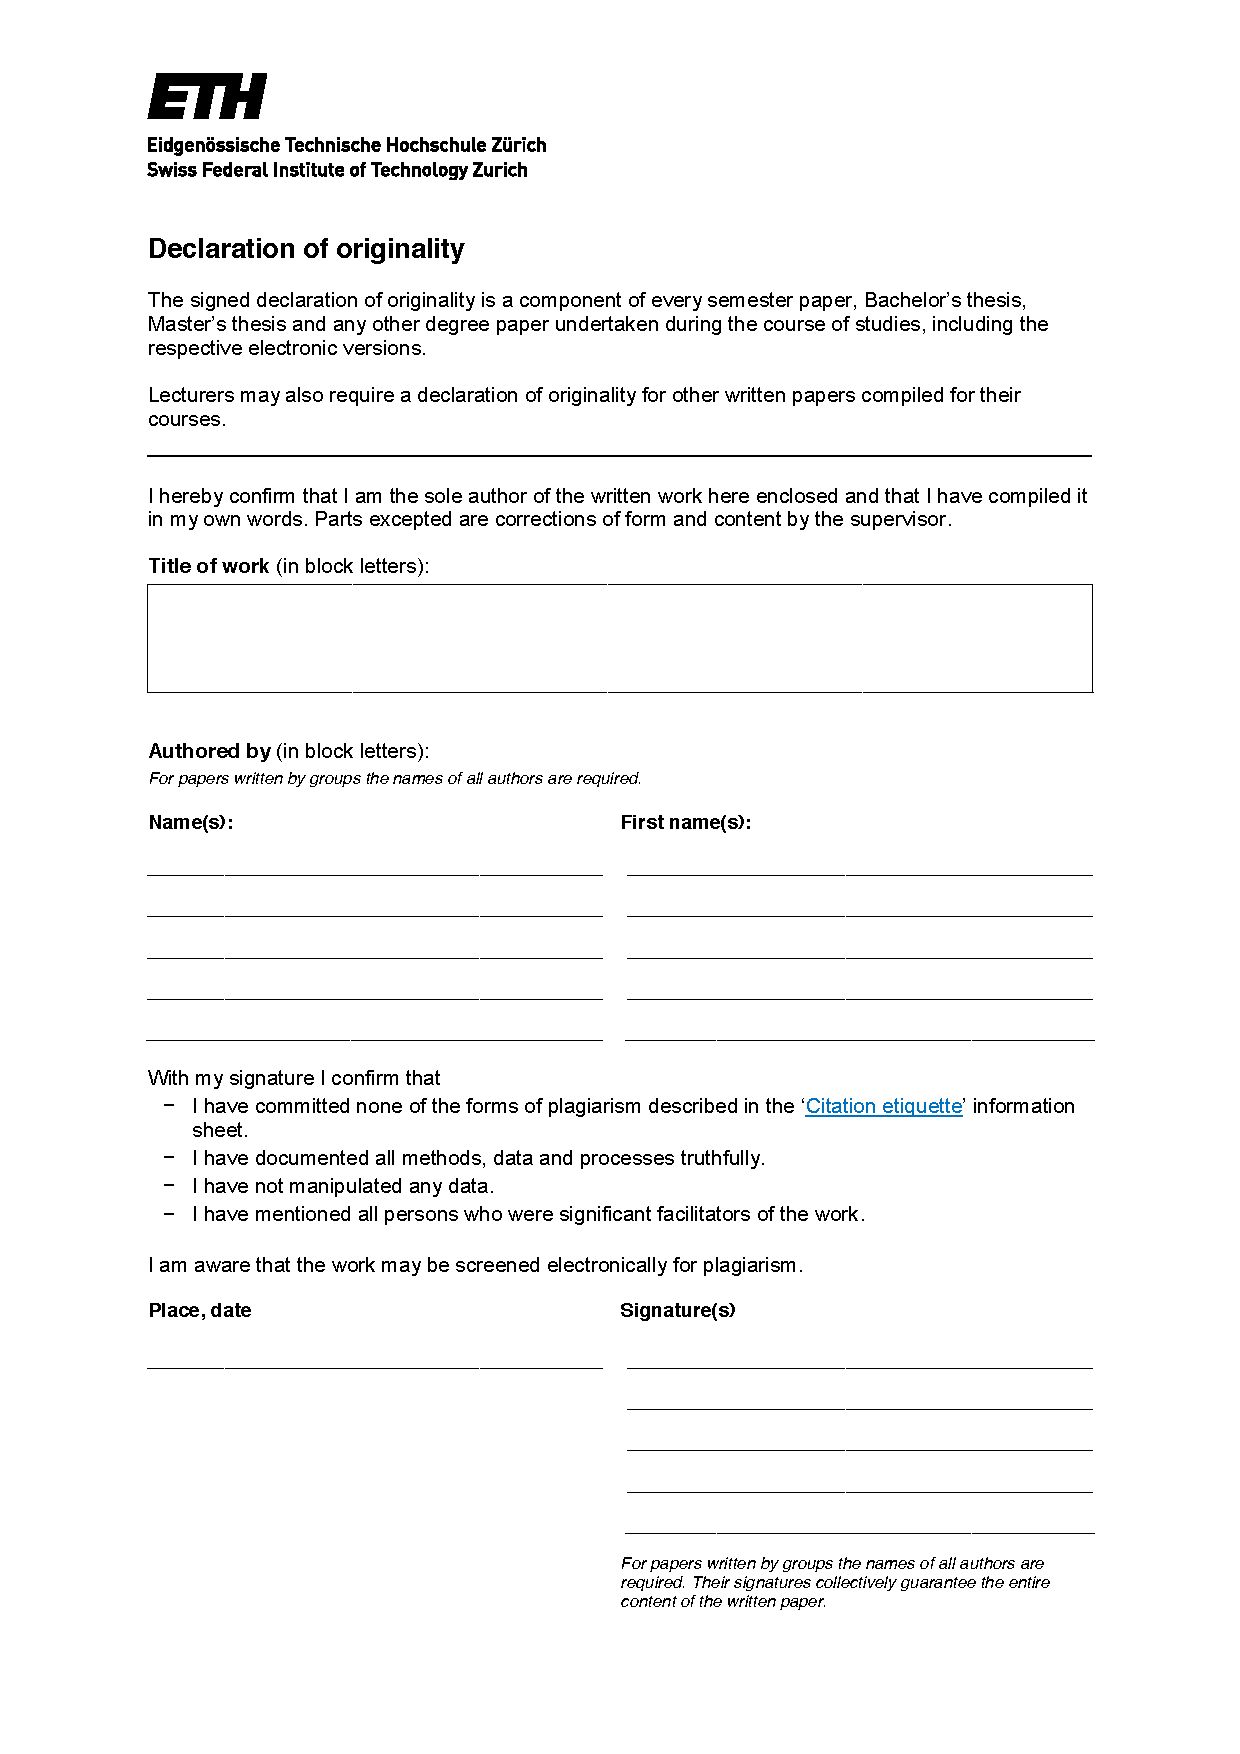
\includepdf[pages={-}]{declaration-originality.pdf}

\end{document}
